\documentclass[12pt]{article}
\usepackage[margin=1in]{geometry}
\usepackage{amsmath,amssymb}
\usepackage{booktabs}
\usepackage{multirow}
\usepackage{graphicx}
\graphicspath{{../scripts/R/kz_passthrough/_outputs/}}
\usepackage[hidelinks]{hyperref}
\usepackage{natbib}
\usepackage{setspace}
\onehalfspacing
\usepackage{caption}
\captionsetup{font=small}

\title{Passing Through: Kazakhstan's Post-2022 Trade Reorientation\\ and the Limits of Value Capture}
\author{Zhanbolat Kakishev\thanks{Nazarbayev University. This paper uses only public data
(UN Comtrade, OECD ICIO, World Bank). Replication code: \texttt{scripts/R/kz\_passthrough/}.
The author previously worked with a consulting team on a related Kazakhstan trade-strategy
engagement; that work is not used here and no confidential material informs this paper.}}
\date{August 2026 \\ \emph{Preliminary draft --- please do not cite}}

\begin{document}
\maketitle

\begin{abstract}
\noindent Since 2022, geopolitical tensions in the region have disrupted direct trade between
Russia and several of its largest partners, and a growing share of that trade is rerouted
through neighbouring economies. This paper documents the reorientation for Kazakhstan at the
product level (HS6, 2018--2025) and asks a question the literature leaves open: how much of
this gross-trade windfall does the host economy retain? In 31 product lines, Kazakhstan's
exports to Russia rose from about \$25m per year before 2022 to roughly \$200m, and its
imports from the EU and China of the same lines roughly tripled; both series break sharply in
the second quarter of 2022 (sup-$F$ of 424 and 329). Yet Kazakhstan re-exports these goods at
a \emph{lower} unit value than it imports them, and---propagating the retained trade margin
through the national input--output table---the domestic value added created per dollar
rerouted is about 8\%, against roughly 76\% for a dollar of domestic manufacturing output.
The customs-duty take is under 1\% of customs revenue, the flow is 0.2--0.3\% of GDP, and
deal-level data show no investment response---no new plant, assembly capacity or logistics
build-out in the sectors the flow passes through. Kazakhstan operates as a corridor, not a
factory: the trade statistics move sharply, the domestic economic footprint far less.

\medskip
\noindent\textbf{Keywords:} trade reorientation, intermediated trade, transit economies,
value added, Kazakhstan, Eurasian Economic Union. \quad \textbf{JEL:} F14, F15, O24, P33.
\end{abstract}

\clearpage

\section{Introduction}

The disruption of direct trade between Russia and its principal partners after February 2022
has produced a visible redirection of trade flows through third countries. Recent work
documents the phenomenon: \citet{chupilkin2026roundabout} show a sharp fall in EU exports to
Russia alongside a matching rise in EU exports to Armenia, Kazakhstan and the Kyrgyz Republic,
with product-level and mirror-statistics evidence of onward movement to Russia;
\citet{chupilkin2025intermediated} quantify the substitution and find it offsets under
10\% of the overall trade impact, though the ratio exceeds one half for many individual
products. This literature establishes \emph{that} rerouting happened and roughly \emph{how
large} it is.

It does not address a distinct question: what does the intermediary economy actually
\emph{gain}? A large increase in gross trade need not translate into domestic value added,
employment or fiscal revenue. If the host merely warehouses and forwards goods that are
produced elsewhere and consumed elsewhere, the domestic economic content of the activity is
limited to a trade-and-transport margin---and that margin may be thin, and understated in the
trade statistics if the outbound leg is under-invoiced. Whether a country in this position is
capturing a windfall or bearing risk for little return is an empirical question with direct
policy relevance, both for the host (is the exposure worth it?) and for the design of the
restrictions the rerouting responds to (are the chokepoints ones where the host retains
little?).

This paper answers that question for Kazakhstan. We build a product-level (HS6) panel of
Kazakhstan's trade with the European Union, China, Turkey and Russia for 2018--2025, using
Kazakhstan's own reports where available and partner ``mirror'' data for the inbound side
(Kazakhstan's import reporting is incomplete for 2020--2022). We identify, from the data, a
``surge basket'' of 31 HS6 lines in which both the inflow from the EU and China and the
outflow to Russia at least doubled after 2022; 25 of the 31 also appear on the EU/US/UK/Japan
list of trade-sensitive items, which we use only as a robustness lens.

We find, first, that the reorientation is large and cleanly timed. Kazakhstan's surge-basket
exports to Russia rose roughly tenfold at the monthly level and break in April 2022; the
inbound flow from the EU and China roughly tripled and breaks in mid-2022. An event study
shows a flat pre-trend, a climb over the first six months after the March-2022 sanctions, and
a plateau thereafter. Armenia and the Kyrgyz Republic show the identical break with no
domestic reform to which it could be attributed, and a placebo basket of civilian goods shows
no comparable movement.

Second, and this is the contribution, Kazakhstan retains little of the gross flow. The
unit value at which Kazakhstan re-exports these goods to Russia is, in the median product,
\emph{below} the unit value at which it imports them, and a regression of the outbound on the
inbound unit value has a slope of 0.27---the price charged to Russia barely tracks the price
paid. Propagating a trade-and-freight margin of the order of 10\% through Kazakhstan's
input--output table, the domestic value added generated per dollar of gross rerouted flow is
about 8\%, against roughly 76\% for a dollar of domestic manufacturing output. The
customs-duty take on the incremental flow is on the order of \$7m per year, under 1\% of
Kazakhstan's customs revenue, and the flow as a whole is 0.2--0.3\% of GDP. Kazakhstan's
national accounts barely register an activity that dominates its trade statistics for these
products.

The paper relates to the sanctions-and-trade literature cited above and, more broadly, to
work on transit and landlocked economies and on the domestic value-added content of trade
\citep{koopman2014tracing,los2016tracing}. Its methodological point is simple: gross trade and
domestic value added can diverge sharply for an intermediary, and the divergence is
measurable with public data and a national input--output table.

\section{Context}

Kazakhstan is a founding member of the Eurasian Economic Union (EAEU), which removes the
customs frontier between Kazakhstan and Russia: goods that clear customs on entry to
Kazakhstan can move onward to Russia without a further border. Kazakhstan is also the land
bridge between China and Russia and, via the Trans-Caspian corridor, between China and Europe.
These features make it a natural conduit for trade that can no longer move directly.

A potential confound is the ``New Kazakhstan'' reform agenda associated with the presidency of
Kassym-Jomart Tokayev, an outward-oriented programme that gathered pace in 2022 with a June
constitutional referendum and a November snap election. A broad liberalisation would raise
trade generally and gradually. We show below that what we observe is instead concentrated in a
narrow set of products, discontinuous at the second quarter of 2022 rather than at any
political-calendar date, absent from a civilian control basket, and mirrored in Armenia and
the Kyrgyz Republic, neither of which had such a reform.

\section{Data}

\paragraph{Trade.} UN Comtrade, HS 6-digit. Annual 2018--2025 for magnitudes; monthly
2019m1--2025m12 (authenticated API) for break timing, the event study and the unit-value
analysis. Kazakhstan stopped reporting monthly to Comtrade after February 2024, so the monthly
series uses 2019--2023 and 2025; 2024 is covered by the annual data and by mirror flows.
We use Kazakhstan's reported exports (complete) and, for the inbound side, the sum of
EU-27, United Kingdom, United States, Japan, Korea, Switzerland and Norway reported exports to
Kazakhstan (``mirror''), because Kazakhstan's own import reports are missing for 2020--2022.

\paragraph{Product sets.} We take 75 HS6 lines: the 50 codes on the February-2024 EU/US/UK/JP
\emph{List of Common High Priority Items} (technology-intensive, potentially dual-use) plus 25
clearly civilian control codes (food, apparel, footwear, furniture, personal care, toys). The
\textbf{surge basket} is defined from the data: the 31 lines in which the mean inflow from the
EU and China and the mean outflow to Russia both at least doubled from 2019--2021 to
2022--2023 (and exceed modest post-period levels). Twenty-five of the 31 are on the priority
list; membership of that list is reported as a robustness check, not used to define the
sample.

\paragraph{Input--output.} OECD Inter-Country Input--Output tables, 2023 edition, Kazakhstan
block, 45 ISIC rev.~4 industries, year 2019. We form the domestic technical-coefficient matrix
$A_d$ from the Kazakhstan-on-Kazakhstan intermediate block, the domestic Leontief inverse
$L_d = (I-A_d)^{-1}$, and the direct domestic value-added coefficients $v_d$; the
domestic value-added multiplier for sector $j$ is $(v_d' L_d)_j$.

\paragraph{Macro.} World Bank World Development Indicators (GDP, reserves, current account,
services value added).

\section{The reorientation}

\subsection{Magnitudes}

Table~\ref{tab:magnitudes} reports the surge basket. Kazakhstan's exports to Russia in these
lines were \$12--37m per year in 2018--2021; they were \$158m in 2022 and about \$200m in
2023--2025. The inbound flow from the EU and China rose from about \$180m per year to \$413m
in 2022 and \$584m in 2023.

\begin{table}[t]
\centering
\caption{Surge-basket trade, USD million per year}
\label{tab:magnitudes}
\begin{tabular}{lrrrrrrrr}
\toprule
 & 2018 & 2019 & 2020 & 2021 & \textbf{2022} & 2023 & 2024 & 2025 \\
\midrule
EU+China $\to$ Kazakhstan (mirror) & 183 & 177 & 173 & 196 & \textbf{413} & 584 & 513 & 445 \\
Kazakhstan $\to$ Russia            &  37 &  32 &  17 &  12 & \textbf{158} & 214 & 175 & 169 \\
\bottomrule
\end{tabular}
\end{table}

\subsection{Timing and the event study}

Monthly, the aggregate surge-basket series break decisively in the second quarter of 2022:
a sup-$F$ statistic of 424 for exports to Russia (Bai--Perron break date 2022m4) and 329 for
the inbound flow (2022m6), against critical values in the low tens. Figure~\ref{fig:monthly}
plots the two series; Figure~\ref{fig:es} the event study, $\text{asinh}(y_t) = \alpha +
\sum_{k\neq -1}\beta_k \mathbf{1}[t-t_0=k] + \varepsilon_t$ with $t_0 = $ 2022m3. Both series
are flat for the fifteen pre-treatment months, climb over the first six post-treatment months,
and plateau---exports to Russia at about $+3.2$ log points, the inbound flow at about $+1$.
The break follows the March-2022 sanctions with a short lag consistent with the time needed to
establish routing; it does not coincide with the 2019 transition, the June-2022 referendum or
the November-2022 election.

\begin{figure}[t]
\centering
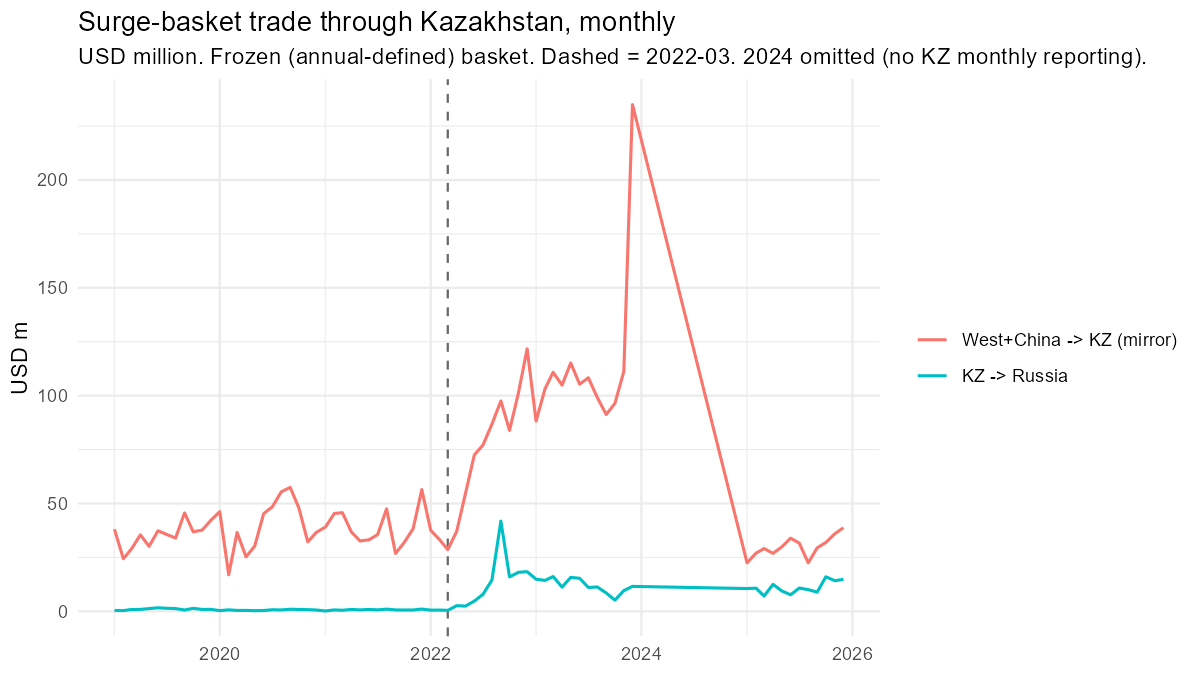
\includegraphics[width=.9\textwidth]{rq1_fig_monthly.png}
\caption{Surge-basket trade through Kazakhstan, monthly. 2024 omitted (no Kazakhstan monthly
reporting). Dashed line: March 2022.}
\label{fig:monthly}
\end{figure}

\begin{figure}[t]
\centering
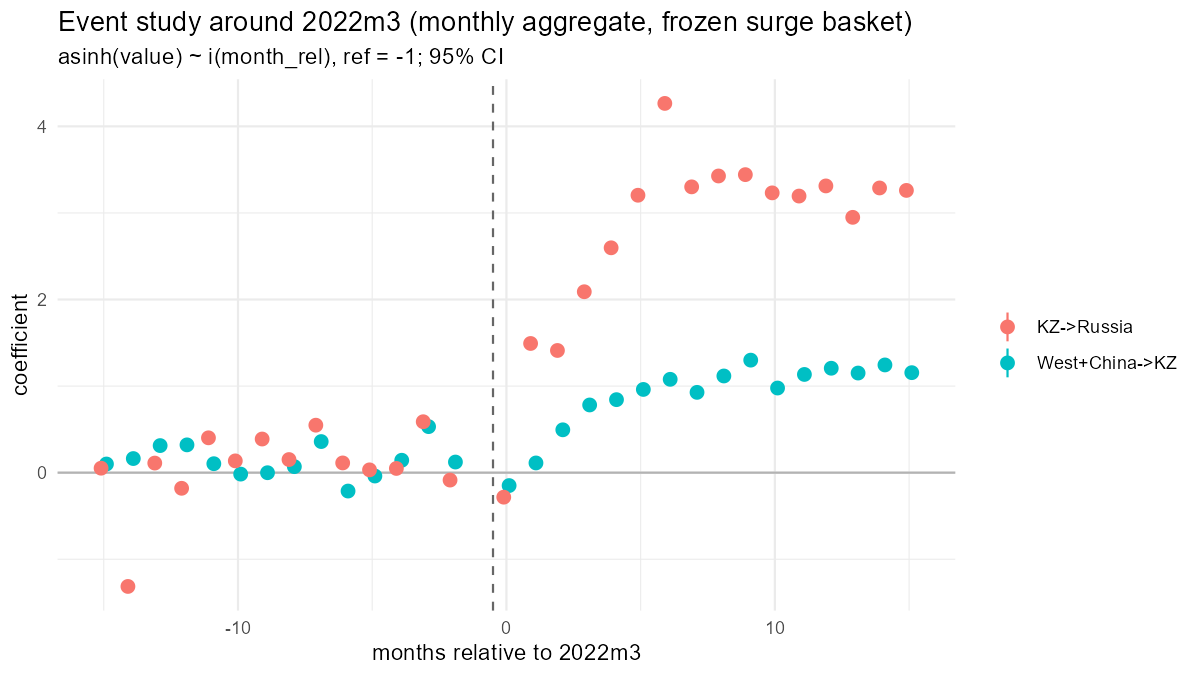
\includegraphics[width=.9\textwidth]{rq1_fig_monthly_eventstudy.png}
\caption{Event study around 2022m3, monthly aggregate, 95\% confidence intervals.}
\label{fig:es}
\end{figure}

\subsection{Difference-in-differences and robustness}

Table~\ref{tab:did} reports $\text{asinh}(y_{it}) = \gamma\,(\text{treated}_i \times
\text{post}_t) + \mu_i + \lambda_t + \varepsilon_{it}$ on the annual panel, with treated the
priority-list codes and controls the civilian basket, HS6 and year fixed effects, and standard
errors clustered by HS6. The point estimates are 2.9 log points for both the inbound flow and
exports to Russia.

\begin{table}[t]
\centering
\caption{Difference-in-differences: priority-list vs.\ civilian controls}
\label{tab:did}
\begin{tabular}{lrr}
\toprule
Outcome (asinh) & $\gamma$ & $p$ \\
\midrule
Kazakhstan imports from the West (reported) & 2.94 & $4.6\times10^{-7}$ \\
Kazakhstan exports to Russia               & 2.88 & $2.3\times10^{-4}$ \\
EU+China $\to$ Kazakhstan (mirror)         & 1.93 & $5.0\times10^{-3}$ \\
\bottomrule
\end{tabular}
\end{table}

Three checks address the reform confound. (i) A placebo difference-in-differences within the
civilian basket, splitting on pre-2022 size, gives $-0.28$ ($p=0.34$); the civilian basket's
own structural break is sup-$F=16$ against $143$ for the surge basket. (ii) Armenia's
surge-basket exports to Russia rose from \$6--11m per year to \$78m in 2022 and \$92m in 2023
(sup-$F=49$); the Kyrgyz Republic's from \$2--4m to \$26m and \$31m (sup-$F=66$). Neither had a
``New Kazakhstan'' reform. (iii) The direction is asymmetric: the inbound surge is from
sanctioning economies, the outbound surge is to Russia.

\section{Value capture}

\subsection{The retained trade margin}

Across the surge basket after 2022, the ratio of Kazakhstan's exports to Russia to its inflow
from the EU and China is 0.43--0.47 in value. For the HS6$\times$month cells with both an
import and a re-export weight ($n=647$), the median ratio of the re-export unit value to the
import unit value is \textbf{0.75} (inter-quartile range 0.30--1.56): Kazakhstan re-exports
these goods, in the median line, at a lower price per kilogram than it paid. A regression of
the log outbound unit value on the log inbound unit value, with HS6 and month fixed effects,
gives a slope of \textbf{0.27} ($p=0.004$)---the outbound price barely tracks the inbound
price. This is consistent with heterogeneous within-HS6 product mix and, plausibly, with
under-invoicing on the outbound leg; either way it is inconsistent with the goods being
transformed or marked up in Kazakhstan. Figure~\ref{fig:wedge} plots the distribution.

\begin{figure}[t]
\centering
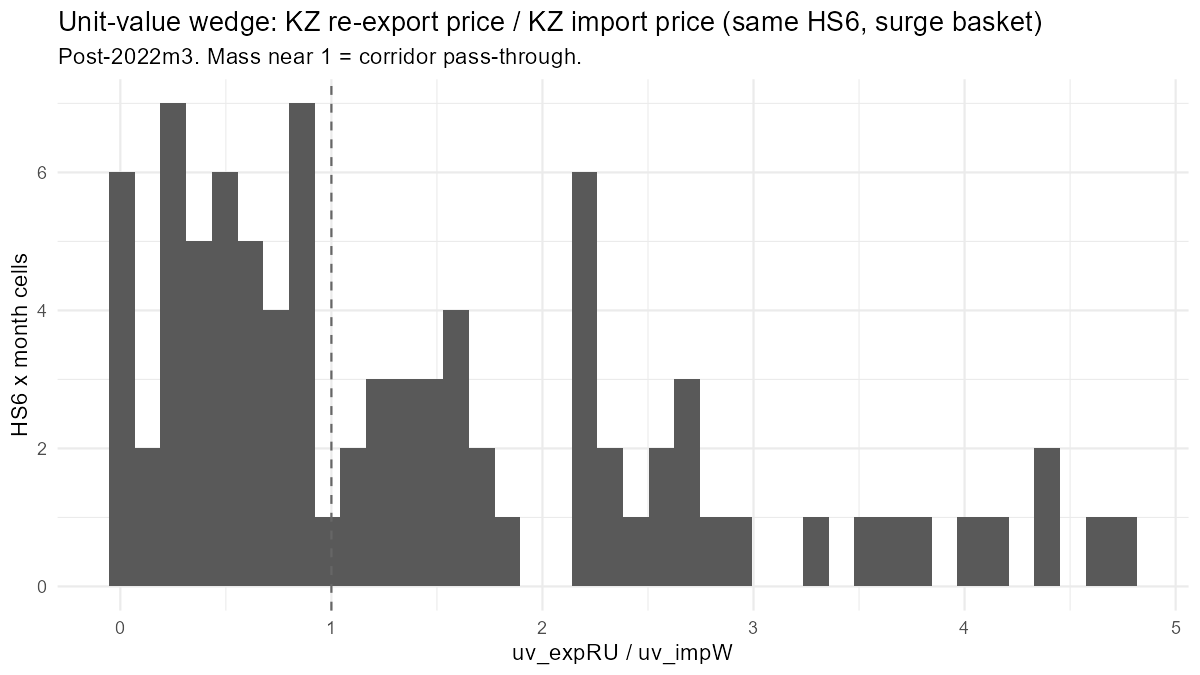
\includegraphics[width=.75\textwidth]{rq2a_fig_wedge_hist.png}
\caption{Unit-value wedge: Kazakhstan re-export price over import price, same HS6, surge
basket, post-2022. Mass near and below 1.}
\label{fig:wedge}
\end{figure}

\subsection{Input--output propagation}

Let $m$ be the trade-and-freight margin retained on a transiting good as a share of its value,
$\bar v^{TT}$ the mean domestic value-added multiplier for Kazakhstan's trade, transport and
warehousing sectors, and $\bar v^{M}$ that for manufacturing. Domestic value added per dollar
of gross rerouted flow is $m\,\bar v^{TT}$; per dollar of domestic manufacturing output it is
$\bar v^{M}$. From the OECD ICIO Kazakhstan block, $\bar v^{TT} = 0.79$ and $\bar v^{M} =
0.76$. Taking $m$ in the range 6--14\% (the Kazakhstan national-accounts convention for
trade, insurance and freight on goods trade), domestic value added per dollar rerouted is
\textbf{5--11\%} (midpoint 8\%), against \textbf{76\%} per dollar of domestic manufacturing
output---a ratio of about \textbf{one to ten}. Of roughly \$560m rerouted to Russia in the
surge basket after 2022, Kazakhstan retains on the order of \textbf{\$44m} as domestic value
added. The conclusion is not sensitive to the multiplier: even at $\bar v^{M}=0.40$ the ratio
is about one to five.

\subsection{Fiscal and macro}

The reorientation-attributable flow---incremental exports to Russia over the pre-2022
baseline---is about \$618m cumulatively over 2022--2025. Customs duty on it, at an EAEU common
external tariff of 4--8\% on the share formally cleared in Kazakhstan, is on the order of
\textbf{\$28m over four years} (\$7m per year); net import VAT is close to zero because the
onward supply to Russia is intra-EAEU and zero-rated. Kazakhstan's annual customs revenue is
of the order of \$4--5bn, so the reorientation adds well under 1\%.

At the macro level the flow is 0.2--0.3\% of GDP. Kazakhstan did record a 2022 current-account
surplus (about \$6.4bn, against deficits before and after), reserve accumulation of \$31bn
over 2023--2025, and services value added up \$63bn over 2022--2024; these are an order of
magnitude too large to be driven by a \$0.6bn-per-year goods-rerouting channel, and are
better explained by energy prices, the reform programme and capital inflows. The reorientation
registers in the trade statistics, not the national accounts.

\section{Does the reorientation induce investment?}

If the reorientation were seeding domestic value addition, we would expect a matching rise in
investment---new plant, assembly capacity, logistics infrastructure---in the sectors the flow
passes through. We test this with deal-level data on mergers, acquisitions and private-equity
and venture transactions in Kazakhstan, 2015--2025 ($n \approx 500$, from Capital~IQ,
PitchBook and Preqin), supplemented by the transaction record of Kazakhstan's state
investment corporation (QIC/Baiterek).

There is no such rise. Classifying deals into value-chain buckets, transactions in
manufacturing of tradeable goods, transport and logistics, and wholesale distribution run at
7.3 per year in 2015--2021 and 7.5 per year in 2022--2025; 2022 itself was the weakest year in
the series (Figure~\ref{fig:mismatch}). Reported deal value in these sectors rises, but is
concentrated in ownership transfers of existing or distressed assets---the ArcelorMittal
Temirtau to Qarmet nationalisation (2023), Eurocopter Kazakhstan and the Lokomotiv rolling-stock
plant (re-nationalisations, 2024), and a \$0.8bn 2025 consolidation of rail-freight and
forwarding assets---not new productive capacity. Greenfield and new-capacity transactions run
at one to two per year throughout. Across the whole 2015--2025 window the data contain
\emph{no} transactions in the specific product lines that dominate the reorientation
(integrated circuits, precision instruments, machinery components): no plant, deal or expansion.

Kazakhstan is adding vehicle assembly (Chinese marques, KIA, \v{S}koda) and some appliance
capacity, but this predates and is largely independent of the reorientation, is kit assembly
with low domestic value added, and serves the domestic and Eurasian consumer market rather
than the flow of restricted components to Russia. The state fund's post-2022 industrial
pipeline is agri-processing and metallurgy, not corridor processing. The one investment
signal that is reorientation-linked---the 2025 rail-freight consolidation, with Russia-linked
asset names---deepens Kazakhstan's role as a forwarding operation, not a producing one.

\begin{figure}[t]
\centering
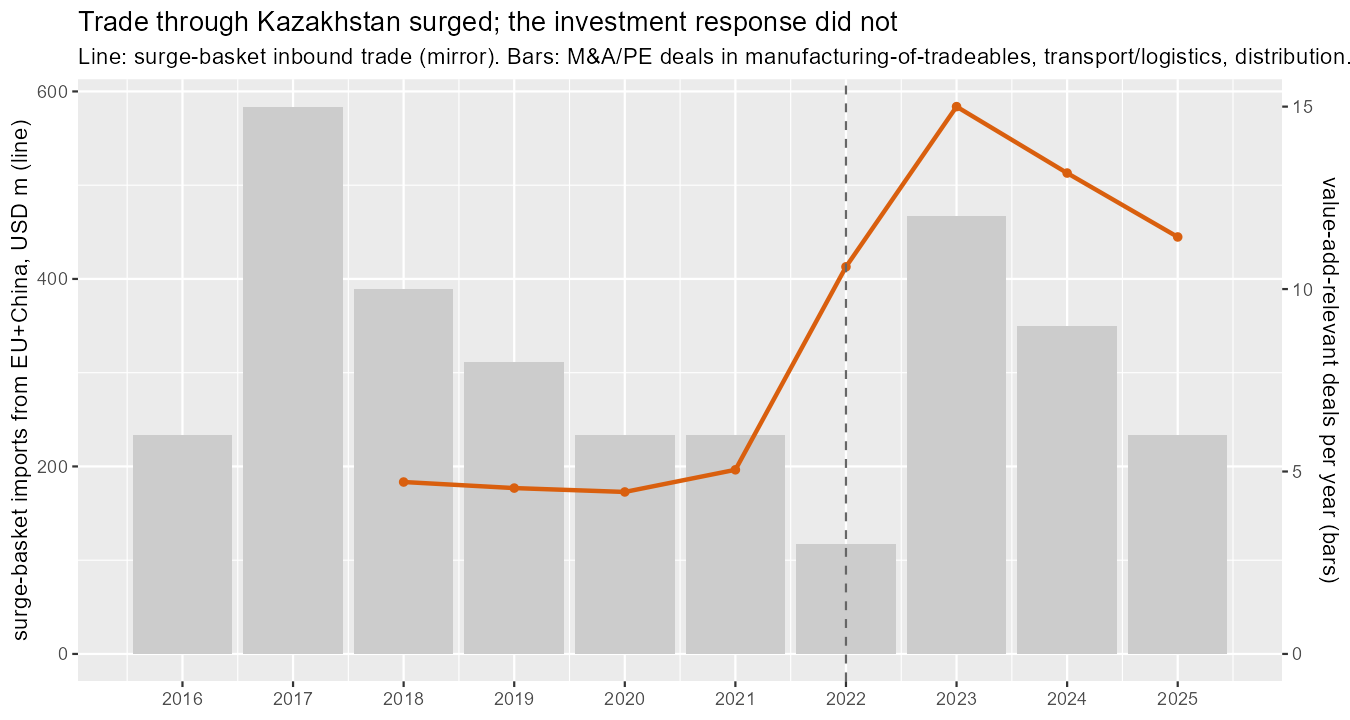
\includegraphics[width=\textwidth]{../scripts/R/kz_valueadd/_outputs/valueadd_fig_mismatch.png}
\caption{Trade through Kazakhstan surged; the investment response did not. Line: surge-basket
inbound trade (mirror), USD million. Bars: annual count of M\&A/PE deals in manufacturing of
tradeables, transport and logistics, and distribution.}
\label{fig:mismatch}
\end{figure}

The mismatch has a simple explanation. Under the Eurasian Economic Union the activity requires
no domestic processing---a good can be imported, warehoused and forwarded untouched, which the
unit-value evidence confirms is what happens. The rents are thin (and partly hidden by
outbound under-invoicing), the flow is expected to be temporary and carries secondary-sanctions
risk, and Kazakhstan's investment climate is weak for growth-stage industrial firms: the
domestic private-equity market has no functioning exit route (buy-back is the leading exit),
capital is dominated by state and development-finance money, and the 2022--25 pipeline is
crowded by nationalisations.

\subsection{Where investment would raise domestic value capture}

The reorientation is nonetheless informative for investment policy, because the trade data
reveal which products have proven demand and proven routes through Kazakhstan. We rank
sectors on a simple index combining the domestic value-added multiplier (from the
input--output table), the import-substitution gap (imports relative to domestic output), the
post-2022 growth in import demand, and the existing deal base, after removing the
surge-basket lines from the electronics-adjacent chapters (Table~\ref{tab:priority}).

Two groups stand out. First, the \textbf{logistics platform}: warehousing and transport
support has among the highest domestic value-added multipliers in the economy (0.82) and is
the corridor's binding constraint; investment here---bonded warehousing, terminals, cold
chain, customs technology---creates domestic value and holds it whether or not the Russia
flow persists. Second, \textbf{import substitution} in machinery, fabricated metal products
and chemicals: Kazakhstan imports six to eight times what it produces in these lines, the
value-added multiplier is around 0.80, and a nascent deal base exists. By contrast, localising
the surge-basket products themselves is the worst option---computer, electronic and optical
manufacturing has the \emph{lowest} value-added multiplier (0.69) and a near-zero domestic
base, and would add sanctions exposure for a temporary flow. The same is true of motor-vehicle
kit assembly.

\begin{table}[t]
\centering
\caption{Sector priority for value-adding investment (index within Kazakhstan)}
\label{tab:priority}
\small
\begin{tabular}{llrrrr}
\toprule
& Sector & VA mult. & Output \$m & Imports/output & Import growth \\
\midrule
\multirow{2}{*}{Platform}
 & Warehousing \& transport support & 0.82 & 6{,}800 & --- & --- \\
 & Wholesale \& retail trade infrastructure & 0.82 & 81{,}000 & --- & --- \\[2pt]
\multirow{3}{*}{Substitution}
 & Machinery \& equipment n.e.c. & 0.80 & 1{,}160 & 8.3 & 1.27 \\
 & Fabricated metal products & 0.81 & 1{,}850 & 1.8 & 1.22 \\
 & Chemicals & 0.79 & 3{,}480 & 1.7 & 1.52 \\[2pt]
\multirow{2}{*}{Avoid}
 & Computer, electronic \& optical (surge basket) & 0.69 & 230 & --- & --- \\
 & Motor vehicles \& parts (kit assembly) & 0.69 & 1{,}530 & 6.1 & 2.55 \\
\bottomrule
\end{tabular}
\end{table}

These opportunities are only investable at scale if the state investment corporation shifts
from lead direct investor to co-investor behind private leads, with larger syndicated tickets
and a credible exit (trade sale or listing) rather than the buy-back that currently dominates.
That is a question about capital-market institutions, which we take up in related work.

\section{Discussion}

For these products, Kazakhstan's trade with Russia and with the West moved by an order of
magnitude after 2022, but the domestic economic content of that movement---value added around
a tenth of the manufacturing equivalent, customs duty under a percent of revenue, a fraction
of a percent of GDP, and no measurable investment response---is small. Kazakhstan is
functioning as a corridor rather than a site of production. For Kazakhstan, this bears on
whether the reorientation is worth its compliance and reputational costs. For the design of
the restrictions the reorientation responds to, it suggests that the intermediary retains
little, so that the economic pressure of enforcement falls mostly on the final buyer and the
original seller rather than on the transit country.

\paragraph{Policy.} Raising domestic value capture is mostly not about attracting the
re-export flow---which adds little value, invites sanctions exposure, and recedes as
enforcement tightens---but about (i) pricing and taxing the transit business Kazakhstan
already has: a published Middle-Corridor service tariff, electronic transit declarations
reconciled against partners' export records to close the under-invoicing leak, and
value-added logistics (bonded warehousing, kitting, quality control) rather than bare
forwarding; (ii) targeting genuine processing only where Kazakhstan has a durable advantage,
with audited rising-local-content conditions rather than nominal ``assembly''; and (iii)
fixing the investment climate---building an exit market, re-orienting state capital toward
co-investment behind private leads, and setting a re-privatisation timetable for the recently
nationalised industrial assets. A fuller treatment is in the companion policy note.

\paragraph{Limitations.} Mirror data for the inbound side; a single input--output vintage
(2019) and the OECD ICIO's relatively high domestic-content shares for Kazakhstan; the trade
margin taken from a national-accounts convention rather than estimated line by line;
under-invoicing on the outbound leg, which biases the retained margin downward and which we can
only bound; and 2024 partial in the monthly data. A robustness appendix using the Kazakhstan
national input--output table (68 products) and line-level tariffs is in progress.

\bibliographystyle{aer}
\bibliography{passthrough}

\end{document}
